\clearpage

\section{結果}
\subsection{励磁電流,電力及び位相差}
入力電圧-励磁電流-電力-電力の関係は\wtab{re1}のようになった.入力電圧上昇とともに電流,電力,位相の増加が確認できる.
	これは電力が電圧,電流に比例するためである.
	\begin{table}[h]
	\centering
	\caption{励磁電流特性}
	\label{tab:re1}
	\begin{tabular}{cccc}
	\hline
	入力電圧$V\,[\rm{V}]$& 電流$i_{0}\,[\rm{A}]$& 電力$P_{0}\,[\rm{W}]$& 位相\,[\rm{deg}]  \\ 
	\hline
	75  & 0.307    & 1.84     & 85.42 \\
	80  & 0.337    & 2.10      & 85.53 \\
	85  & 0.378    & 2.36     & 85.79 \\
	90  & 0.429    & 2.64     & 86.08 \\
	95  & 0.483    & 2.96     & 86.30 \\
	100 & 0.552    & 3.34     & 86.53 \\ \hline
	\end{tabular}
	\end{table}
	
\subsection{励磁電流波形の計測}
入力電圧が$80\,\rm{V}, 100\,\rm{V}$時の励磁電流をそれぞれ\wpfig{1}に示す.

$100\,\rm{V}$の場合の方が$80\,\rm{V}$の場合と比べて波形が正弦波に近いことがわかる.また,ひずみが発生している部分も少ない.
\begin{figure}[h]
	\centering
	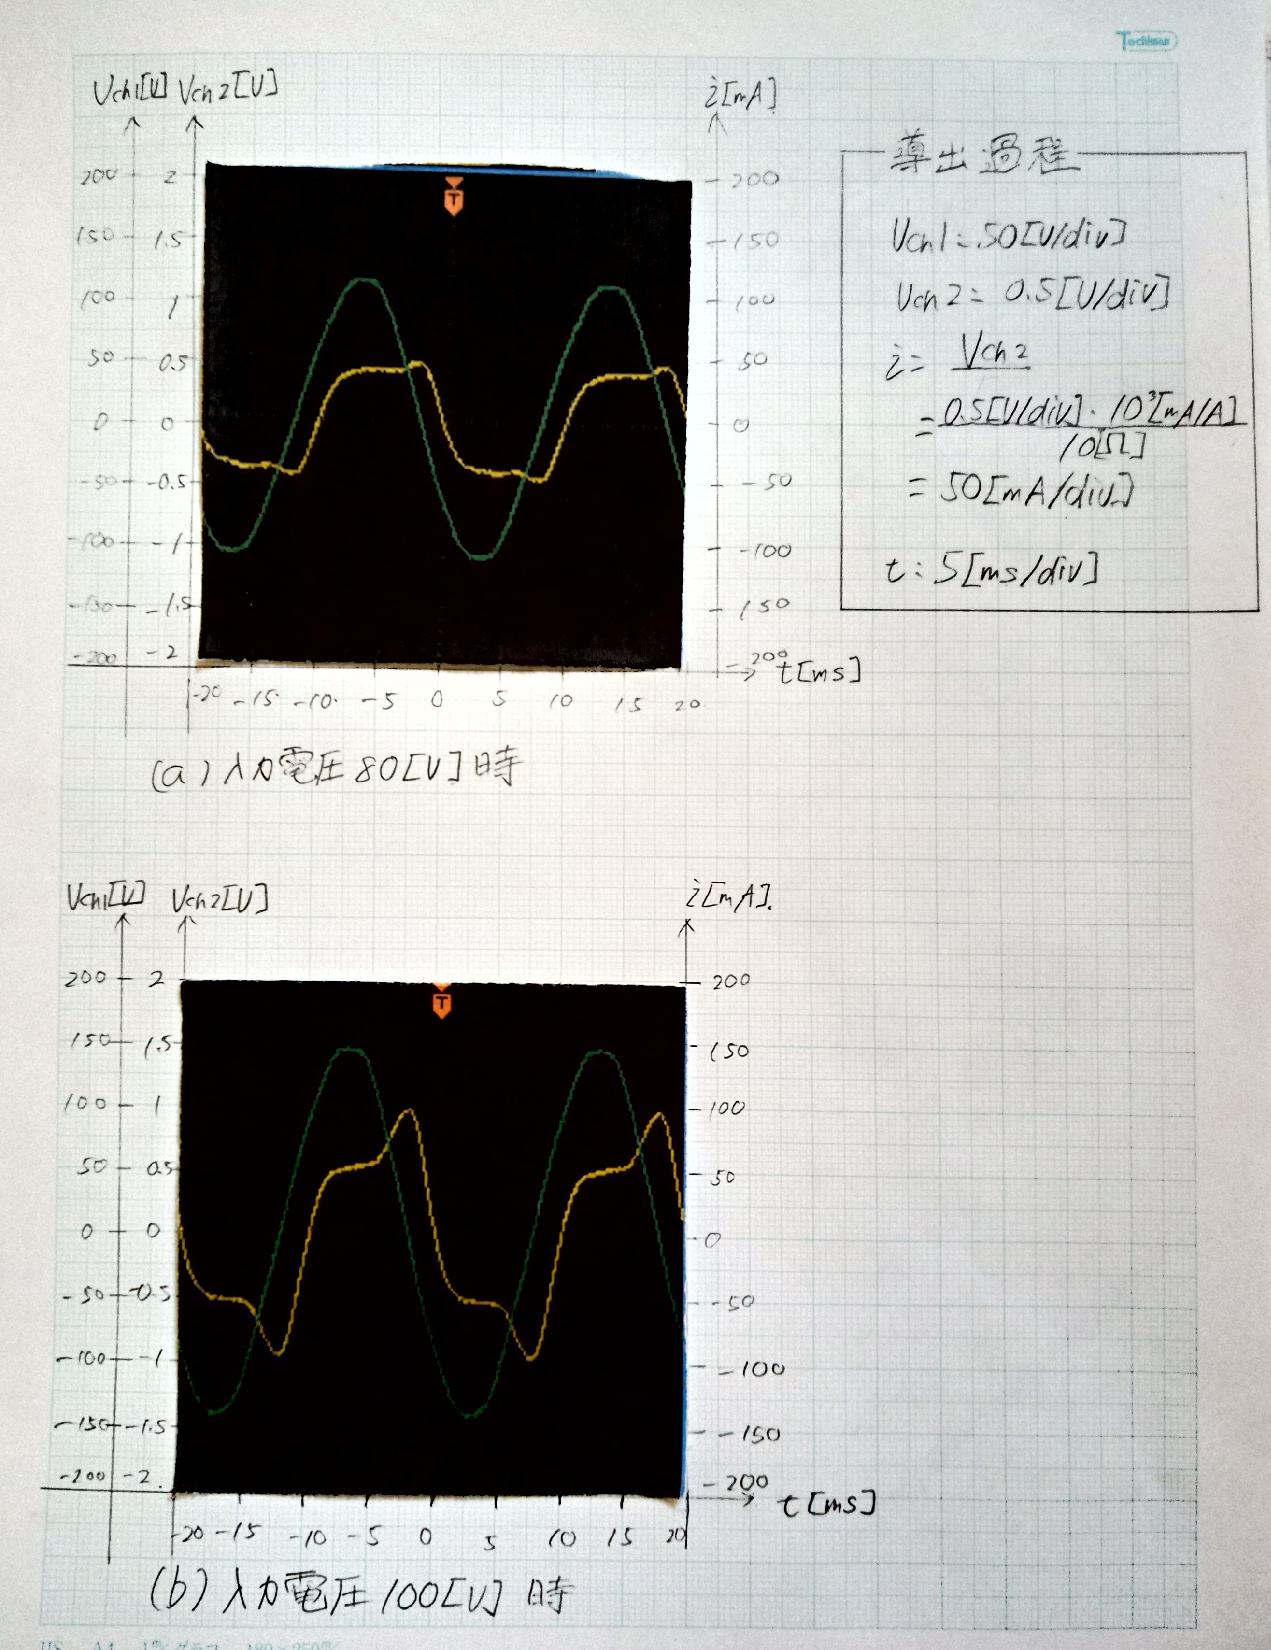
\includegraphics[scale=0.8]{./data/graph/1.pdf}
	\caption{励磁電流}
	\label{fig:1}
\end{figure}

\subsection{ヒステリシスループの計測}
入力電圧が$80\,\rm{V}, 100\,\rm{V}$時のヒステリシスループをそれぞれ\wpfig{2}に示す.

$100\,\rm{V}$の場合では,$80\,\rm{V}$の場合に比べ飽和状態に近く,保磁力,飽和磁束密度がともに大きいことがわかる.
\begin{figure}[h]
	\centering
	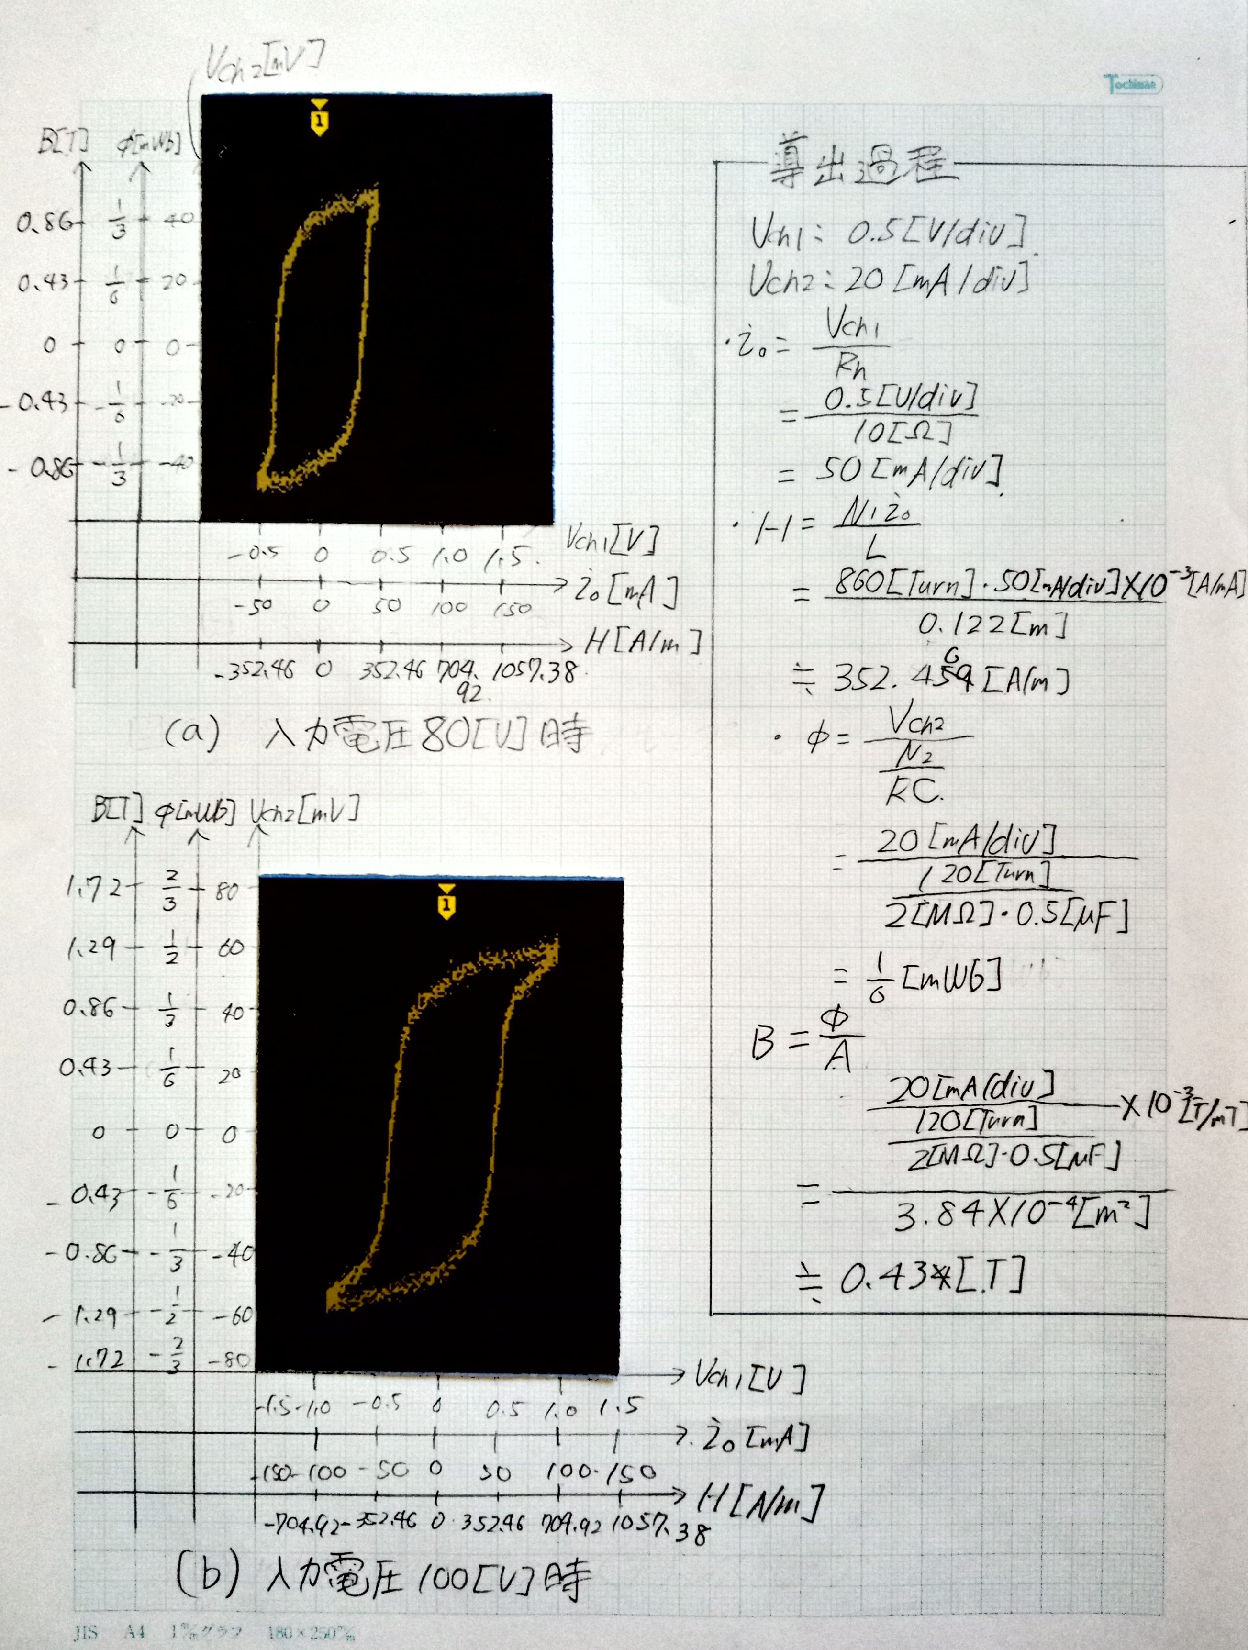
\includegraphics[scale=0.8]{./data/graph/2.pdf}
	\caption{ヒステリシスループ}
	\label{fig:2}
\end{figure}

\subsection{励磁電流作図}
ヒステリシスループを用いて作図した励磁電流を\wpfig{3}に示す.

この図からも励磁電流のひずみが発生していることが確認できる.また積分回路により位相がずれている影響により,それぞれの波形の位相が異なっていることがわかる.

\begin{figure}[h]
	\centering
	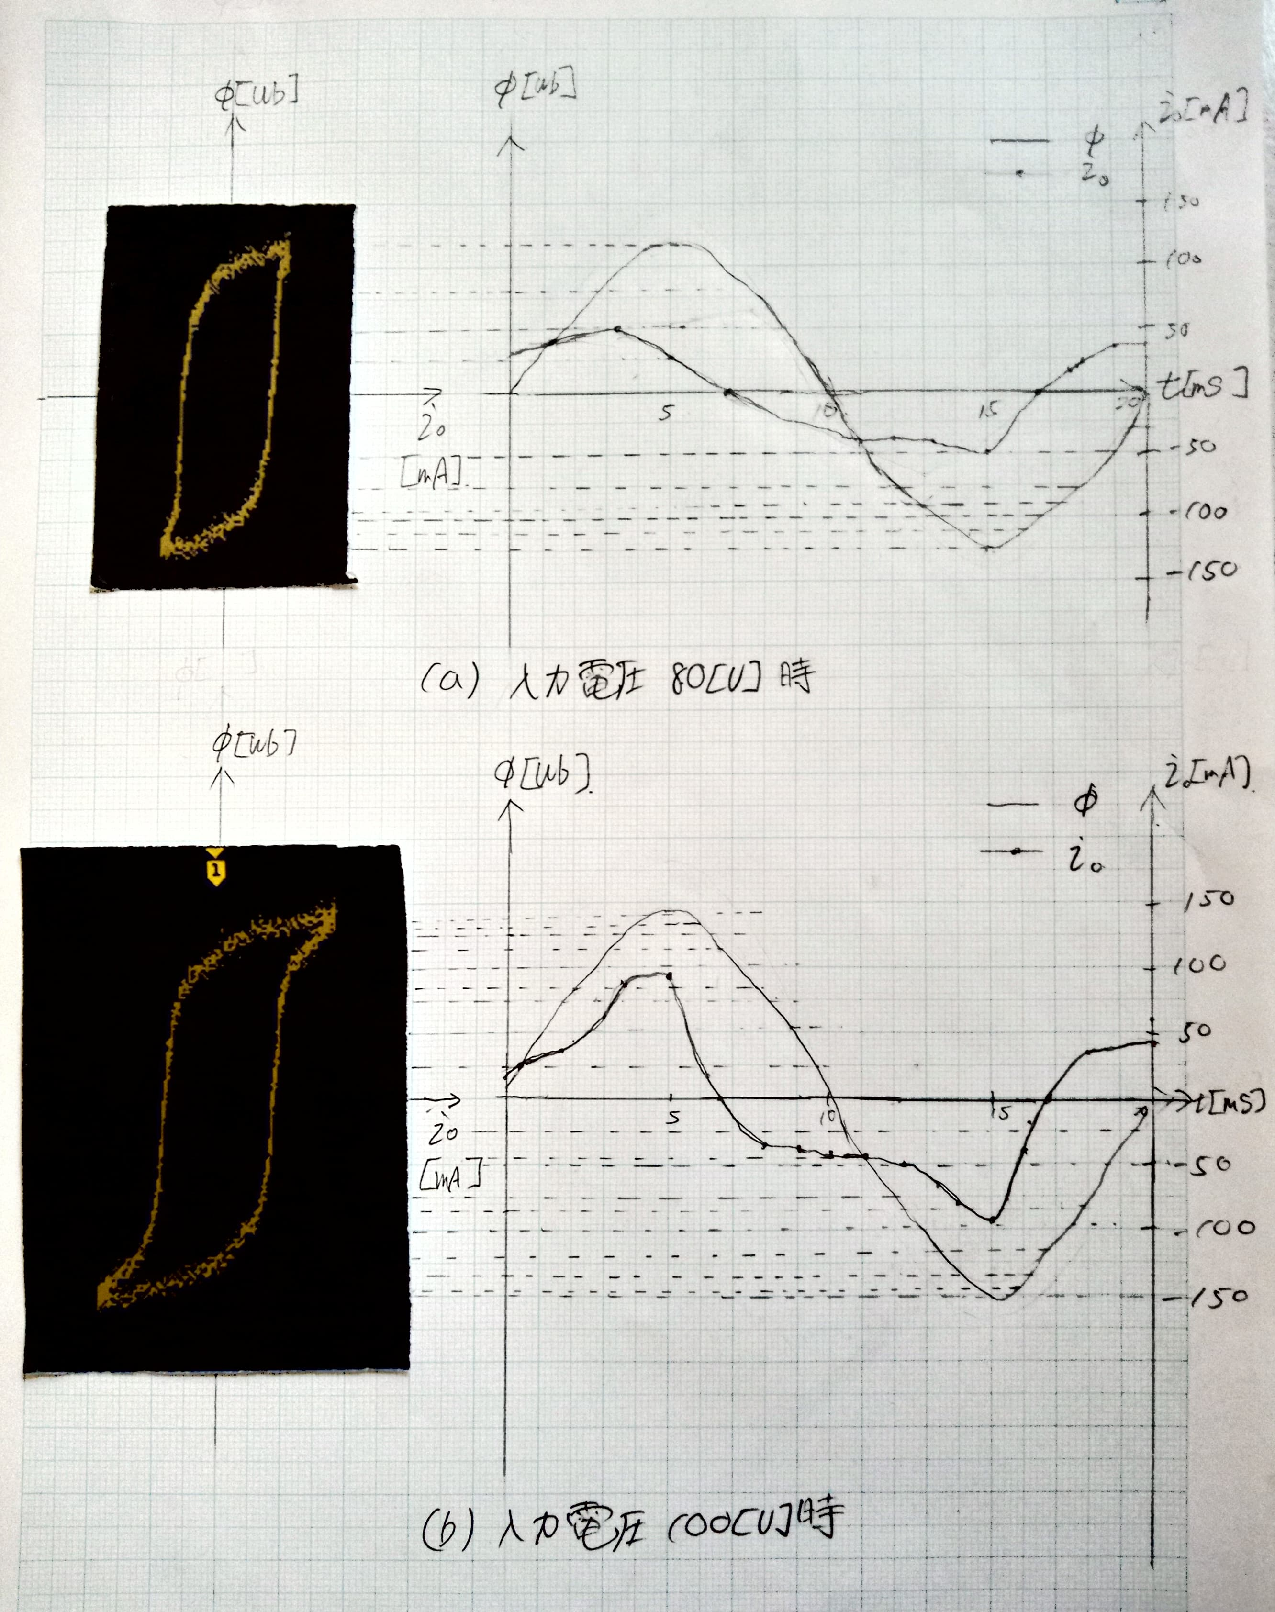
\includegraphics[scale=0.8]{./data/graph/3.pdf}
	\caption{ヒステリシスループを用いて作図した励磁電流}
	\label{fig:3}
\end{figure}